\documentclass[a4paper,14pt,russian]{extreport}
%\documentclass[tikz,14pt,russian]{standalone}
% Third parameter is needed for TOC displaying (why?)
\usepackage{../common/dsturep} % оформление по ДСТУ 3008-95
\usepackage{import}
\usepackage{standalone}
\usepackage{comment}
\usepackage{bbm}

\usepackage{tikz}
\usepackage{tikz-3dplot}
\usetikzlibrary{calc}
\usetikzlibrary{plotmarks}
\usepackage{pgfplots}

%\usepackage{scrextend}
\usepackage{changepage}
\usepackage{caption}
\usepackage{listings}
%\usepackage[title,titletoc]{appendix}
%\usepackage{appendix}
\usepackage{longtable}
%\usepackage{slashbox}
\usepackage{diagbox}
\usepackage{lscape}
\usepackage{algorithmic}
\usepackage{algorithm}

\newcommand{\indicatorof}[1]{\mathbbm{1}_{#1}}
\newcommand{\indicator}[1]{\mathbbm{1}\!\left( #1 \right)}
\newcommand{\Indicator}[1]{\mathbbm{1}\!\left\{ #1 \right\}}
\newcommand{\probability}[1]{\mathbb{P}\left( #1 \right)}
\newcommand{\Probability}[1]{\mathbb{P}\left\{ #1 \right\}}
\newcommand{\cdfof}[2]{F^{#1}\left(#2\right)}
\newcommand{\cdf}[1]{\cdfof{}{#1}}
\def\Tau{\mathrm{T}}
\newcommand{\meanof}[2]{\operatorname{M}_{#1} #2}
\newcommand{\Meanof}[2]{\meanof{#1}{\left[ #2 \right]}}
\newcommand{\mean}[1]{\meanof{}{#1}}
\newcommand{\Mean}[1]{\Meanof{}{#1}}
\newcommand{\dispersionof}[2]{\operatorname{D}_{#1} #2}
\newcommand{\Dispersionof}[2]{\dispersionof{#1}{\left[ #2 \right]}}
\newcommand{\dispersion}[1]{\dispersionof{}{#1}}
\def \mcond {\;\middle|\;}
\newcommand{\Covergencen}[1]{\xrightarrow[#1\to\infty]{}}
\newcommand{\cov}[1]{\operatorname{cov}\!\left( #1 \right)}
\DeclareMathOperator*{\argmax}{arg\,max}
\DeclareMathOperator*{\argmin}{arg\,min}

\newcommand{\drawHist}[1]{\begin{tikzpicture}[scale=1]
  \begin{axis}[ymin=-5, ymax=5, xmin=5, xmax=30, ytick=\empty,
    xmajorgrids={true},
    ylabel={Кількість точок}, ylabel near ticks,
    xlabel={час, с}]

\draw[dashed,color=gray!50] ({rel axis cs:0,0}|-{axis cs:0,0}) -- ({rel axis cs:1,0}|-{axis cs:0,0});
\addplot table [x, y, col sep=comma] {data/#1.csv};
\end{axis}
\end{tikzpicture}}

\captionsetup[subfigure]{skip=0ex} % global setting for subfigure

\usepackage{stringenc}
\usepackage{pdfescape}

\makeatletter
\renewcommand*{\UTFviii@defined}[1]{%
  \ifx#1\relax
    \begingroup
      % Remove prefix "\u8:"
      \def\x##1:{}%
      % Extract Unicode char from command name
      % (utf8.def does not support surrogates)
      \edef\x{\expandafter\x\string#1}%
      \StringEncodingConvert\x\x{utf8}{utf16be}% convert to UTF-16BE
      % Hexadecimal representation
      \EdefEscapeHex\x\x
      % Enhanced error message
      \PackageError{inputenc}{Unicode\space char\space \string#1\space
                              (U+\x)\MessageBreak
                              not\space set\space up\space
                              for\space use\space with\space LaTeX}\@eha
    \endgroup
  \else\expandafter
    #1%
  \fi
}
\makeatother
\DeclareUnicodeCharacter{00AD}{-}

\def\chapterConclusion{\section*{Висновки до розділу \arabic{chapter}}
\addcontentsline{toc}{section}{Висновки до розділу \arabic{chapter}}}

\def\male{male}
\def\female{female}


%\input{../common/minted.inc}   % оформление листингов в minted
%\bibliographystyle{../common/utf8gost705u}
%\bibliographystyle{../common/utf8gost71u}
\bibliographystyle{../common/utf8gost780u}
%\bibliographystyle{plain}

\usepackage[square,numbers,sort&compress]{natbib}
\renewcommand{\bibnumfmt}[1]{#1.\hfill} % нумерация источников в самом списке — через точку
%\renewcommand{\bibsection}

\usepackage{glossaries}
\makeglossaries

\def\passYear{2016}
\def\faculty{физико-технический институт}
\def\department{Кафедра информационной безопасности}
\def\departmentHead{Н. В. Грайворонский}
\def\kind{Дипломна робота}
\def\level{магістр}
\def\specialityCode{8.04030101}
\def\specialityTitle{Прикладная математика}
\def\theme{Наука про данные: обмен результатами и начальный анализ}
\def\gender{female}
\def\mentorGender{male}
\def\course{2}
\def\group{ФИ-41}
\def\name{Лавягина Ольга Алексеевна}
\def\mentorRank{}
\def\mentorName{Колотий Андрей Всеволодович}
\def\reviewerRank{Rank}
\def\reviewerName{Name}
\def\subject{Специальные разделы программирования}


\usepackage{csvsimple}

\begin{document}

\import{1_title/}{title.tex}

\clearpage

\pagenumbering{gobble}
%\import{3_abstract/}{main.tex}

%\pagestyle{empty}
%\thispagestyle{empty}
%\tableofcontents

\clearpage
\pagenumbering{arabic}
\pagestyle{fancy}
\setcounter{page}{2}

\clearpage

\chapter{Данные}

Материалы для лабораторной работы были получены на геопортале геологической служды США --- USGS \cite{USGS}. Скачанный архив содержит каналы изображений. Каждое изображение космических аппаратов (КА) серии Landsat имеет уникальный идентификатор, структура которого следующая:

[Идентификатор сенсора и КА (3 символа)] + [Координаты снимка в WRS-2-системе (Path, Row, 6 символов)] + [Год] + [DOY] + [Режим съёмки (5 символов)].

Например, LC81810252015048LGN00 --- снимок КА Landsat-8, полученный сенсором OLI/TIRS; координаты снимка в системе WRS-2 --- 818 (Path) 102 (Row), съёмка проведена 48-го дня 2015 года, режим съёмки LGN00. Содержание архива с продуктом уровня обработки  данного снимка изображено на рисунке \ref{archive}. 

\begin{figure}[h]
  \centering
  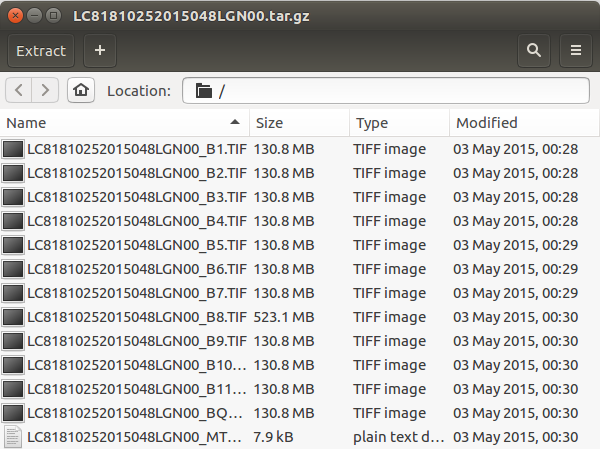
\includegraphics[width=.75\textwidth]{archive.png}
  \caption{Архив с продуктом обработки дынных КА Landsat-8 OLI/TIRS уробня обратотки L1T}
\label{archive}
\end{figure}


\chapter{Задание}

Средствами командной строки операционной чистемы, а также с помощью бинариев библиотеки GDAL разработать автоматический сценарий, который будет совершать обработку данных дистанционного зондирования Земли (ДЗЗ), соответственнос поставленными заданиями.

Задание 1. Распаковка набора архивов с продуктами ДЗЗ в новосозданные папки, названия которых будут соответствовать идентификаторам изображения.

Задание 2. Конкатинация каналов видимого, ближнего и среднего инфракрасного спектрального диапазонов изображения в единственный GEOTIFF файл.

Задание 3. Перепроектирование спутникового изображения в указанную картографическую систему координат.

Задание 4. Конкатинация изображений двух соседних <<row>> с одинаковым <<path>>.

Задание 5. Обрезка результирующего изображения по заданному векторному контуру.

Ход выполнения работы. Получить архивы с сутниковыми изображениями, и файл с векторным контуром для дальнейшей обрезки. Средствами командной строки операционной системы (без ограничения в выборе ОС) и с использованием бинариев библиотеуи GDAL создать программный сценарий для автоматической обработки спутниковых изображений согласно поставленным заданиям. 

\chapter{Листинг кода}


\chapter*{Выводы}
\addcontentsline{toc}{chapter}{Выводы}

\clearpage
\phantomsection
\addcontentsline{toc}{chapter}{Список литературы}
\renewcommand\bibname{Список литературы}
\bibliography{bibliography.bib}

\end{document}
